\documentclass[a4paper]{article}
%% Language and font encodings
\usepackage[english]{babel}
\usepackage[utf8x]{inputenc}
\usepackage[T1]{fontenc}
\usepackage[numbers]{natbib}
\usepackage[a4paper,%
						top=3cm,%
						bottom=2cm,%
						left=3cm,%
						right=3cm,%
						marginparwidth=1.75cm]{geometry}
%% Useful packages
\usepackage{amsmath,amsthm,amssymb,amsfonts,enumerate}
\usepackage{graphicx}
\usepackage[colorinlistoftodos]{todonotes}
\usepackage[colorlinks=true, allcolors=blue]{hyperref}
\usepackage{booktabs}
%
\newtheorem{theorem}{Theorem}
\newtheorem{lemma}{Lemma}
\newtheorem{definition}{Definition}
\newtheorem{assumption}{Assumption}
\newtheorem{remark}{Remark}
\newtheorem{example}{Example}
\newtheorem{proposition}{Proposition}
%
\newcommand{\R}{\mathbb{R}}
\newcommand{\N}{\mathbb{N}}
\newcommand{\s}{\subseteq}
\newcommand{\e}{\varepsilon}
%
%
%
%%title
\title{
	Existence, characterization, and simulation
	of optimal control policies in some classical epidemic models
}
%
\author{Saul, Frank, David}
%
\begin{document}
<<<<<<< HEAD
	\maketitle
=======
\maketitle

\begin{abstract}
	Your abstract.
\end{abstract}

\section{Introduction}

{\bf Notation}. Each element $x$ in $\R^n$ is written as a column vector and $x^\top$ denotes the transpose. We write the gradient of $g:\R^n\to\R$ as a row vector 
    \[ g_x =(\partial g/\partial x_1,\ldots, \partial g/\partial x_n). \]
If $\lambda:\R\to\R^n$ is differentiable, the derivative is denoted $\dot{\lambda}=(d\lambda^1/dt,\ldots,d\lambda^n/dt)^\top$. The Jacobian matrix of $f=(f^1,\ldots,f^n)^\top:\R^n\to\R^n$ is   
\[f_x=\begin{bmatrix}
f^1_x\\
f^2_x\\
\vdots \\
f^2_x
\end{bmatrix}\]

\section{Optimal control problems}

	\subsection{Deterministic OCPs in continuous time}

Let $X\s\R^n$ and $U\s \R^m$ be nonempty sets. The sets $X$ and $U$ are 
respectively called the {\it state space} and the {\it control space}. Consider 
the following {\it control system}
\begin{equation}\label{CoDiffEq}
\dot{x}(t)=f(t,x(t),u(t)),\qquad t\in[0,T], \quad x(0)=x_0.
\end{equation}
where $f:[0,T]\times X\times U\to \R^n$ and $u:[0,T]\to U$. 
%In order to guarantee the existence of a solution $x$ to \eqref{CoDiffEq}, 
%we need the following.

\begin{assumption}\label{Assum1}  The function $f:[0,T]\times X\times U\to \R^n$
is measurable and there exists a constant $L>0$ such that
\begin{eqnarray}
  |f(t,x,u)-f(t,x_1,u)| & \leq & L|x-x_1|\label{LipfInx}
  %\\|f(t,0,u)| & \leq & L\label{fBound}
\end{eqnarray}
for every $x,x_1\in X$, $t\in[0,T]$, and $u\in U$.
\end{assumption}

%A proof of the following result can be found, for instance, in Yong \cite[Sect. 2.1]{Yong2015}. 

\begin{theorem}\label{ExAdmisPair} 
	Under Assumption \ref{Assum1}, the system 
	\eqref{CoDiffEq} has a unique 	solution $x_u$ for each measurable function 
	$u:[0,T]\to U$. %The solution $x_u$ satisfies	\begin{equation}\label{ineqSol} 
	%	|x_u(t)|\leq e^{Lt}(1+|x_0|) -1,\qquad t\in [0,T].	\end{equation}
\end{theorem}
\begin{proof} 
Let $w(s):=e^{Lt}$, $t\in [0,T]$, and consider the vector space 
    \[X=\{x:[0,T]\to \R^n\mid f \mbox{ is continuous}\}\] 
with the norm
    \[ \|x\|_w:=\sup_{t\in[0,T]} \frac{|x(t)|}{w(t)}. \]
It can be shown, with a slight modification in \cite[Section 2.1]{Teschl}, that the pair $(X,\|\cdot\|_w)$ is a Banach space. We claim that the operator $K:X\to X$ given by 
    \[ K[x](t):=x_0 + \int_0^t f(s,x(s),u(s))ds\]
is a contraction with contraction constant $1-e^{-LT}$. Indeed, 
    \begin{eqnarray*}
    \| K[x] - K[y] \|_w & = & \sup_{t\in[0,T]} \frac{|\int_0^t [f(s,x(s),u(s)) -f(s,y(s),u(s))]ds|}{w(t)}\\
        & \leq &   \sup_{t\in[0,T]} \frac{L\int_0^t w(s)[w(s)]^{-1}|x(s) -y(s)|ds}{w(t)}\\
        &\leq &  L\|x-y\|_w \sup_{t\in[0,T]} \frac{\int_0^t w(s)ds}{w(t)}\\
        & = &  L\|x-y\|_w \sup_{t\in[0,T]}\frac{[e^{Lt}-1]/L}{e^{Lt}}\\
        & = &  (1-e^{-LT})\|x-y\|_w. 
    \end{eqnarray*}
Therefore by Banach's fixed point theorem \cite[Theorem 2.1]{Teschl}, there exists a unique $x\in X$ satisfying \eqref{CoDiffEq}.
\end{proof}


	Given a measurable function $u$, let $x_u(\cdot)$ denote the solution to 
\eqref{CoDiffEq}. The terminal point $x_u(T)$ can be constrained to belong to a 
set $M\s X$, in such a case we assume the following. 

\begin{assumption} Let $M$ be a nonempty subset of $X$. 
	The set of {\it admissible controls} 
	\begin{equation}\label{FeasCont}  
		 U_M:=\{u:[0,T]\to U\mid u\  
		 \mbox{\rm is measurable and } x_u(T)\in M\} 
	\end{equation}
	is nonempty. A pair $(x_u,u)$, where $u\in U_M$, is called an 
	{\it admissible pair}. To ease notation, we simply write $(x,u)$.
\end{assumption}


Consider the {\it performance index} of an admissible control $u$, given the initial state $x_0$, 
        \begin{equation}\label{PiBolza} V(u,x_0) := \int_0^Tg(t,x(t),u(t))\,dt + h(x(T)),\end{equation}
where $g:[0,T]\times X\times U\to \R$ and $h:X\to\R$ are measurable.

The {\it optimal control problem} (OCP) consists of finding an admissible control $u^\ast$ such that
\[ V(u^\ast,x_0)=\sup\{ V(u,x_0)\mid u\in U_M \}.\]
If there exists such a control $u^\ast$, then it is called an {\it optimal policy} or {\it optimal control}. The pair $(x^\ast,u^\ast)$, where $x^\ast$ is guaranteed by Theorem \ref{ExAdmisPair}, is called an {\it optimal pair}.



\begin{remark}\rm
The performance index \eqref{PiBolza} is said to be in the {\it Bolza form}. When $g= 0$ and $h\neq 0$, it is said to be in the {\it Mayer form}. Another form occurs when $h= 0$ and $g\neq 0$; in such a case, \eqref{PiBolza} is said to be in the {\it Lagrange form}. These three forms are equivalent; see, for instance, Cesari \cite[Sect. 1.9]{Cesari83}. 
\end{remark} 

%%------------------------------------------------------------------------------

\subsection{Existence of optimal policies}




\begin{assumption}
The functions $g$ and $h$ in the performance index \eqref{PiBolza}
 
\end{assumption}










%%------------------------------------------------------------------------------
\subsection{The maximum principle}


The following lemma is a classical result in Calculus of Variations. We give a proof for completness.

\begin{lemma}\label{VariatLemma} Let  

\end{lemma}




%%------------------------------------------------------------------------------
\subsection{Sufficient conditions}









\section{Classic epidemic models}
[Saúl]

>>>>>>> e679d59816eaa68703488a39a82d53239597dac1

	\begin{abstract}
		Your abstract.
	\end{abstract}
%
	\section{Introduction}
	\section{Optimal control problems}
		\subsection{Deterministic OCPs in continuous time}

Let $X\s\R^n$ and $U\s \R^m$ be nonempty sets. The sets $X$ and $U$ are 
respectively called the {\it state space} and the {\it control space}. Consider 
the following {\it control system}
\begin{equation}\label{CoDiffEq}
\dot{x}(t)=f(t,x(t),u(t)),\qquad t\in[0,T], \quad x(0)=x_0.
\end{equation}
where $f:[0,T]\times X\times U\to \R^n$ and $u:[0,T]\to U$. 
%In order to guarantee the existence of a solution $x$ to \eqref{CoDiffEq}, 
%we need the following.

\begin{assumption}\label{Assum1}  The function $f:[0,T]\times X\times U\to \R^n$
is measurable and there exists a constant $L>0$ such that
\begin{eqnarray}
  |f(t,x,u)-f(t,x_1,u)| & \leq & L|x-x_1|\label{LipfInx}
  %\\|f(t,0,u)| & \leq & L\label{fBound}
\end{eqnarray}
for every $x,x_1\in X$, $t\in[0,T]$, and $u\in U$.
\end{assumption}

%A proof of the following result can be found, for instance, in Yong \cite[Sect. 2.1]{Yong2015}. 

\begin{theorem}\label{ExAdmisPair} 
	Under Assumption \ref{Assum1}, the system 
	\eqref{CoDiffEq} has a unique 	solution $x_u$ for each measurable function 
	$u:[0,T]\to U$. %The solution $x_u$ satisfies	\begin{equation}\label{ineqSol} 
	%	|x_u(t)|\leq e^{Lt}(1+|x_0|) -1,\qquad t\in [0,T].	\end{equation}
\end{theorem}
\begin{proof} 
Let $w(s):=e^{Lt}$, $t\in [0,T]$, and consider the vector space 
    \[X=\{x:[0,T]\to \R^n\mid f \mbox{ is continuous}\}\] 
with the norm
    \[ \|x\|_w:=\sup_{t\in[0,T]} \frac{|x(t)|}{w(t)}. \]
It can be shown, with a slight modification in \cite[Section 2.1]{Teschl}, that the pair $(X,\|\cdot\|_w)$ is a Banach space. We claim that the operator $K:X\to X$ given by 
    \[ K[x](t):=x_0 + \int_0^t f(s,x(s),u(s))ds\]
is a contraction with contraction constant $1-e^{-LT}$. Indeed, 
    \begin{eqnarray*}
    \| K[x] - K[y] \|_w & = & \sup_{t\in[0,T]} \frac{|\int_0^t [f(s,x(s),u(s)) -f(s,y(s),u(s))]ds|}{w(t)}\\
        & \leq &   \sup_{t\in[0,T]} \frac{L\int_0^t w(s)[w(s)]^{-1}|x(s) -y(s)|ds}{w(t)}\\
        &\leq &  L\|x-y\|_w \sup_{t\in[0,T]} \frac{\int_0^t w(s)ds}{w(t)}\\
        & = &  L\|x-y\|_w \sup_{t\in[0,T]}\frac{[e^{Lt}-1]/L}{e^{Lt}}\\
        & = &  (1-e^{-LT})\|x-y\|_w. 
    \end{eqnarray*}
Therefore by Banach's fixed point theorem \cite[Theorem 2.1]{Teschl}, there exists a unique $x\in X$ satisfying \eqref{CoDiffEq}.
\end{proof}


	Given a measurable function $u$, let $x_u(\cdot)$ denote the solution to 
\eqref{CoDiffEq}. The terminal point $x_u(T)$ can be constrained to belong to a 
set $M\s X$, in such a case we assume the following. 

\begin{assumption} Let $M$ be a nonempty subset of $X$. 
	The set of {\it admissible controls} 
	\begin{equation}\label{FeasCont}  
		 U_M:=\{u:[0,T]\to U\mid u\  
		 \mbox{\rm is measurable and } x_u(T)\in M\} 
	\end{equation}
	is nonempty. A pair $(x_u,u)$, where $u\in U_M$, is called an 
	{\it admissible pair}. To ease notation, we simply write $(x,u)$.
\end{assumption}


Consider the {\it performance index} of an admissible control $u$, given the initial state $x_0$, 
        \begin{equation}\label{PiBolza} V(u,x_0) := \int_0^Tg(t,x(t),u(t))\,dt + h(x(T)),\end{equation}
where $g:[0,T]\times X\times U\to \R$ and $h:X\to\R$ are measurable.

The {\it optimal control problem} (OCP) consists of finding an admissible control $u^\ast$ such that
\[ V(u^\ast,x_0)=\sup\{ V(u,x_0)\mid u\in U_M \}.\]
If there exists such a control $u^\ast$, then it is called an {\it optimal policy} or {\it optimal control}. The pair $(x^\ast,u^\ast)$, where $x^\ast$ is guaranteed by Theorem \ref{ExAdmisPair}, is called an {\it optimal pair}.



\begin{remark}\rm
The performance index \eqref{PiBolza} is said to be in the {\it Bolza form}. When $g= 0$ and $h\neq 0$, it is said to be in the {\it Mayer form}. Another form occurs when $h= 0$ and $g\neq 0$; in such a case, \eqref{PiBolza} is said to be in the {\it Lagrange form}. These three forms are equivalent; see, for instance, Cesari \cite[Sect. 1.9]{Cesari83}. 
\end{remark} 

%%------------------------------------------------------------------------------

\subsection{Existence of optimal policies}




\begin{assumption}
The functions $g$ and $h$ in the performance index \eqref{PiBolza}
 
\end{assumption}










%%------------------------------------------------------------------------------
\subsection{The maximum principle}


The following lemma is a classical result in Calculus of Variations. We give a proof for completness.

\begin{lemma}\label{VariatLemma} Let  

\end{lemma}




%%------------------------------------------------------------------------------
\subsection{Sufficient conditions}







	\section{Classic epidemic models}
	[Saúl]
	\section{Control Policies in Epidemics}
	[Saúl]
    	  Here we present  several control models that we consider as good 
examples. Before talking about this good examples, we give the core of optimal 
policy modeling, see for example the survey of \citet{Wickwire1977}, for more
details.

  First, we require a model to describe the spreading of an uncontrolled
disease, and whose transitions generate a cost. Then, we add a continuous
control action to modify the changes from one state to another but in such way
that the mentioned cost is optimized. A rule that prescribes which control
operation to use at each time, is a control policy. A control policy which
applies only information from the current state of the controlled system to
prescribe control actions is a \emph{closed-loop} or \emph{feedback} control.
If the current state is not observable, or the control function only depends 
on the time we have an \emph{open-loop} policy: the sort of policies that we 
consider in this work.

  Here, we consider control policies that affect the bounded rates at which
population moves from one class (e.g., infected) to another (e.g., recovered).
In all these problems, the control function appears linearly in the relevant
dynamic. Next, we specify a cost functional which assigns the total cost of the
control policy implementation. Then the problem is to determine a policy that
optimizes the regarding cost strategy.

  Now we present the mentioned good examples. In what follows $X$ denotes a 
vector with all concerning populations, for example, according to SIR model 
\eqref{eqn:sir_model},  $X=(S, I, R)^\top$ .

	    \subsection{Vaccination}
	    	\section{Standard SIR model with logistic grow}
We use the standard population model with logistic grow reported
\cite{Schaefer2009}, see table for parameter description. To introduce the 
vaccination and treatment as mitigation control policies, we firs deal with the
uncontrolled dynamics described by:
\begin{equation}\label{eqn:SIR}
	\begin{aligned}
		\frac{dS}{dt} &=
			\mu N  
			- \beta \frac{S I}{N} 
			- \mu \frac{N}{K} S ,
		\\
		\frac{dI}{dt} &=
			\beta \frac{S I}{N}
			- (\gamma + \delta) I
			- \mu \frac{N}{K} I,
		\\
		\frac{dR}{dt} &= 
			\gamma I 
			- \mu \frac{N}{K} R ,
		\\
		S(0) &= S_0, \quad
		I(0) = I_0, \quad
		R(0) = R_0,
		\\
		N &= S + I +R,
		\\
		\frac{dN}{dt} &=
			\mu N 
			\left(
				1 - \frac{N}{K}
			\right).
	\end{aligned}
\end{equation}

Given initial population sizes $S_0, I_0, R_0$, the goal is to determine the best policy to
mitigate the outbreak described by the SIR model \eqref{eqn:SIR} and optimize a regarding  cost. In this context, the policies are Lebesgue measurable bounded functions
which optimize a given convex functional cost. For example, \citeauthor{Schaefer2009} pursue to minimize the infected population described by \eqref{eqn:SIR} while minimizing the cost of vaccination $u_1$ and treatment $u_2$. In symbols, the authors seek to minimize the objective functional
\begin{equation}
	\label{eqn:sir_logistic}
  \begin{aligned}
      & \int_{0}^T	
    		\left[
    			B_1 I(t) 
    			+ B_2 \left[\frac{R(t)}{K}\right]^m [u_1(t)]^2 + B_3 [u_2(t)]^2
    		\right] dt,
    		\qquad  m\geq 1,
      \\
    \text{subject to}
  \\
    \frac{dS}{dt} &=
			\mu N  
			- \beta \frac{S I}{N} 
			- \mu \frac{N}{K} S - u_1(t) S,
		\\
		\frac{dI}{dt} &=
			\beta \frac{S I}{N}
			- (\gamma  + \mu + \delta) I 
			- \mu \frac{N}{K} I
			- u_2(t) I,
		\\
		\frac{dR}{dt} &= 
			\gamma I 
			- \mu \frac{N}{K} R 
			+ u_1(t) S 
			+ u_2(t) I,
		\\
		S(0) &= S_0, \quad
		I(0) = I_0, \quad
		R(0) = R_0. \quad
	\end{aligned}
\end{equation}
%
%
Here $S$, $I$, $R$ respectively denotes the epidemiological
compartments for susceptible, infected and recover classes. Note 
that entire population $N=S+I+R$ obeys the logistic growth described by the
last equation of model \eqref{eqn:SIR}. \Cref{tbl:sir_logistic} encase a 
description and the values used to obtain \Cref{fig:figure1sirlog}.

\begin{table}[htb]
  \begin{center}
    \begin{tabular}{@{}rll@{}} 
      \toprule
      &
      \multicolumn{1}{c}{\textbf{Description}}
      & 
      \multicolumn{1}{c}{\textbf{Value}}
      \\
        \midrule
        $\beta$
          & Incidence rate
          & \SI{0.05}{day^{-1}}
      \\
      $\gamma$
        & Infect time
        & \SI{0.1}{day^{-1}}
      \\
      $\mu$
        & Intrinsic growth rate
        & \SI{0.00004}{day^{-1}}
      \\
        $K$
        & Carrying capacity
        & \num{5000}
      \\
      $\delta$
        & Death rate due to disease
        & \SI{0.1}{day^{-1}}
      \\
      \\  
      $B_1$,$B_2$,$B_3$
        & Weight for infected population,
        & \num{1.0}, \num{100}, \num{1000}
        \\
        & vaccination, and treatment 
      \\
      $u_1^{\max}, u_2^{\max}$
        & Max vaccination and treatment 
        \\
        & rates
        & \SI{0.1}{day^{-1}}, \SI{0.6}{day^{-1}}
      \\
      \\
      && \textbf{Initial Conditions}
      \\
      \cmidrule{3-3}
      && $S_0 = \SI{4500}{humans}$
      \\
      && $I_0 = \SI{499}{humans}$
      \\
      && $R_0 = \SI{1}{human}$
      \\
      \bottomrule
    \end{tabular}
    \caption{Parameter description and simulation values for the optimal problem
      \eqref{eqn:sir_logistic}
    }
    \label{tbl:sir_logistic}
	\end{center}
\end{table}
%
\begin{figure}
  \centering
  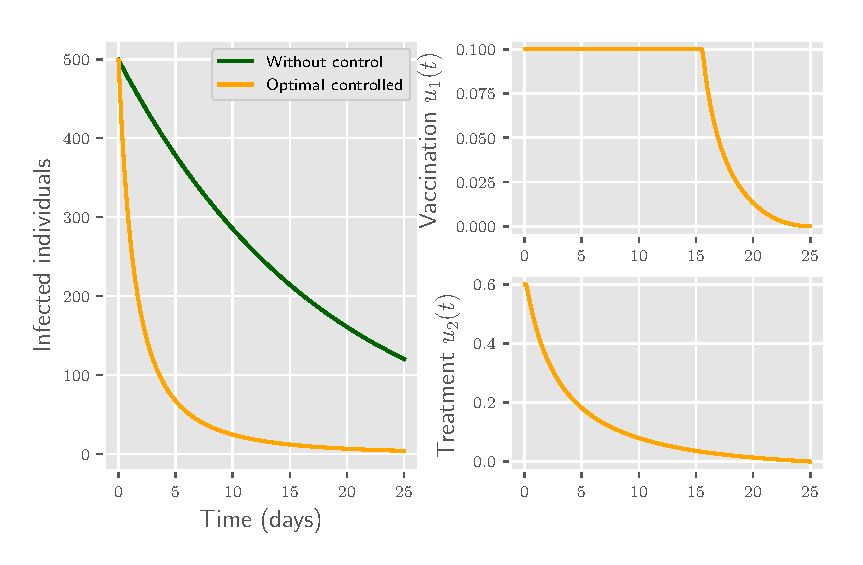
\includegraphics{Figures/figure_1_sir_log}
  \caption{}
  \label{fig:figure1sirlog}
\end{figure}


	    \subsection{Treatment}
	    	\subsection*{Two-strains Tuberculosis}
Seeking to reduce the latent and infectious groups with the 
resistant-strain tuberculosis, in \cite{Lenhart2002} the authors  use 
control theory to describe optimal strategies in a tuberculosis model 
which considers the effect of treatment in two kinds of strains. The 
controlled version reads:
	\begin{equation}\label{eqn:MDR-TB_model}
	  \begin{aligned}
	    \frac{dS}{dt} &=
		    \Lambda - \beta_1 S \frac{I_1}{N} 
		    - \beta_3 S \frac{I_2}{N}
		    \mu S,
		  \\
		  \frac{L_1}{dt} &=
			  \beta_1 S \frac{I_1}{N}
			  - (\mu + k_1) L_1
			  - u_1 (t) r_1 L_1
			  + (1 - u_2 (t)) p r_2 I_1
				+ \beta_2 T \frac{I_1}{N}
				- \beta_3 L_1 \frac{I_2}{N},
			\\
			\frac{I_1}{dt} &= 
				k_1 L_1
				- (\mu + d_1) I_1
				-r_2 I_1,
			\\
			\frac{L_2}{dt} &=
				(1 - u_2(t)) q r_2 I_1
				- (\mu + k_2) L_2
				+ \beta_3 (S + L_1 + T) \frac{I_2}{N},
			\\
			\frac{I_2}{dt} &=
				k_2 L_2 - (\mu + d_2) I_2,
			\\
			\frac{d T}{dt} &=
				u_1(t) r_1 L_1
				+ (1 - (1 - u_2(t))(p + q)) r_2 I_1
				- \beta T \frac{I_1}{N}
				- \beta_3 T \frac{I_2}{N}
				-\mu T.
	  \end{aligned}
	\end{equation}

	\citeauthor*{Lenhart2002} consider time dependent 
optimal control strategies associated with \emph{case holding} and 
\emph{case finding}. They incorporate the case finding control by 
adding a term which identifies and  cure a fraction 
of latent individuals. Case finding consequently reduces the 
rate of disease development by latent individuals. The authors include 
case holding by adding a term which may decrease the 
treatment failure rate of individuals with sensitive  TB, so, this 
control reduce the incidence of drug resistant TB. In model 
\eqref{eqn:MDR-TB_model}, $u_1$ denotes the fraction of typical TB 
latent individuals that is identified  and will put under treatment 
\textemdash case finding control\textemdash and 
$1 - u_2$ represents the effort that prevents the failure treatment in 
typical TB infectious individuals.

	The controls $u_1$ ,$u_2$ reduce the latent and infected 
groups with resistant TB. However, the case holding and the case finding 
strategies produce a economic fee. In \cite{Lenhart2002} the authors use
\begin{equation}\label{eqn:MDR-TB_action}
	 J(u_1, u_2) =
		 \int_0 ^ {t_f}
			 \left[
				 L_2(t) + I_2(t) 
				 + \frac{B_1}{2} [u_1(t)] ^ 2
				 + \frac{B_2}{2} [u_2(t)] ^ 2
			 \right]dt,
\end{equation}
to describe the regarding cost.
%
%
\begin{table}[htb]
  \centering
  \begin{tabular}{rllrl}
    \toprule
       \multicolumn{5}{c}{\textbf{Description}}\\
        \midrule
        $\beta_1$ 
            & Probability that a susceptible 
        &&
          $r_1$ 
            & 
            Treatment recover rate of 
        \\
         & individual becomes infected.
           &&&
            individuals with latent TB.
        \\
        $\beta_2$ 
          & Probability that a recovered 
        && 
          $r_2$ 
            &
            Treatment rate recover of 
          \\
          & individual  become infected
            &&&
              individuals with infectious TB.
          \\
        $\beta_3$ 
          & Probability that a uninfected 
          &&
          $p$, $q$
          & 
            Proportion of infectious individuals 
          \\
          & individual become infected 
            &&&
              that not complete the treatment
            \\
          & by resistant-TB 
            &&&
              for TB or MDR-TB respectively.
      \\
      \\
        $\mu$ 
          & Natural per-capita death rate.
          &&
            $N$ 
            &
              Total population size.
      \\
        $d_1$ 
          & Per-capita death rate by TB.
          &&
            $\Lambda$
            & Recruitment rate.
              
          \\
      $d_2$ 
          & Per-capita  death rate by MDR-TB.
          &&
            $t_f$ 
              & Final time.
          \\
      \\
      $k_1$ 
        & Rate at which an latent TB 
        &&
          $B_1$ 
            &
              Systematic cost of the
        \\
        & individual becomes infectious. 
          &&&
            case finding  control.
      \\
          $k_2$  
          & Rate at which an latent individual
          &&
            $B_2$
            & 
            Cost of the case holding strategy
          \\
          & with MDR-TB becomes infectious.
    \\
    \bottomrule
    \end{tabular}
  \caption{Parameters description and simulation values for the control 
  problem \eqref{eqn:MDR-TB_model}.}
  \label{tbl:parameters_MDR-TB_model_des}
\end{table}

%

	    \subsection{Quarantine}
	    	
\subsection*{SARS}
  If an emergent disease lacks of a rapid diagnostic test, therapy or vaccine,
then isolation and quarantine of individuals exposed to the disease
seems an obvious control policy. For example \citet{Gumel2004} model
strategies of this kind for the severe acute respiratory syndrome (SARS).
SARS was a highly contagious and viral disease emerged in China late in 
\num{2002}  and quickly spread to \num{32} countries and regions causing more than \num{774} deaths and \num{8098} infections worldwide.

Based in the work of \citet{Gumel2004}, \citeauthor{Yan2008} report in 
\cite{Yan2008} a control epidemic model for SARS. They use quarantine and 
isolation as mitigation controls. The authors also propose sub-optimal control 
policies and perform numerical simulations with genetic algorithms. The 
controlled version used in the mentioned 
reference reads:
%
%
\begin{equation}\label{eqn:sars_model}
	\begin{aligned}
		\dfrac{dS}{dt} &=
			\Lambda 
			-\dfrac{
				S
				\left(
					\beta I 
					+ \mathcal{E}_E  \beta E
					+ \mathcal{E}_Q  \beta Q
					+ \mathcal{E}_J  \beta J
				\right)
			}{N}
			- \mu S,
		\\
		\dfrac{dE}{dt} &=
			p +
			\dfrac{
				\beta S
				\left(
					\beta I 
						+ \mathcal{E}_E \beta E
						+ \mathcal{E}_Q \beta Q
						+ \mathcal{E}_J \beta J
				\right)
			}{N}
			-(
				u_1(t) + k_1 + \mu
			)E,
		\\
		\dfrac{dQ}{dt} &=
			u_1(t) E 
			- (k_2 + \mu) Q,
		\\
		\dfrac{dI}{dt} &=
			k_1 E 
			-(u_2(t) + d_1  + \sigma_1 + \mu) I,
		\\
		\dfrac{dJ}{dt} &=
			u_2(t) I 
			+ k_2 Q
			- (d_2 + \sigma_2 + \mu) J,
		\\
		\dfrac{dR}{dt} &=
			\sigma_1 I
			+\sigma_2 J
			- \mu R.
	\end{aligned}
\end{equation}
The control variable $u_1$ denotes the proportion of people in quarantine 
who had contact with an infected person inside of a quarantine program or
educational campaigns. Control $u_2$ models the proportion of symptomatic 
population which is in an isolation program. The authors consider the 
following epidemiological classes.
\begin{table}[h!]
	\begin{center}
		\begin{tabular}{@{}rll@{}} 
			$S$: & Susceptible individuals 
			\\
			$E$: & Asymptomatic individuals who have been 
			\\
			   & exposed to the virus but have not yet developed 
			\\
			   & clinical symptoms of SARS 
			\\
			$Q$: & Quarantine individuals
			\\
			$I$: & Symptomatic 
			\\
			$J$: & Isolated
			\\
			$R$: & Recovered
			\\
				& $N = S + E + Q + I + J + R$.
		\end{tabular}
	\end{center}
\end{table}
We enclose a description of the model parameters 
in \Cref{tbl:sars_table_des}.
So, giving the disease dynamics in \eqref{eqn:sars_model}, the problem is to 
minimize the functional cost
\begin{equation}\label{eqn:sars_cost}
  V(X, u)
    = \int_{0}^{t_f}
      \left[
        B_1 E(t)
        + B_2 Q(t)
        + B_3 I(t)
        + B_4 J(t)
        + \frac{C_1}{2} u_1^2 (t)
        + \frac{C_2}{2} u_2^2 (t)
      \right]
      dt.
\end{equation}
Here, parameter $B_i$ denotes the linear cost of the infected 
class and $C_1, C_2$ are the costs for isolation and quarantine controls, respectively.
\Cref{tbl:sars_table_des} displays a description of the regarding parameters.
%
\begin{table}[H]
    \begin{center}
      \begin{tabular}{@{}rl@{}}
        \toprule
        & \multicolumn{1}{l}{\bf{Parameter Description}}
        \\
        \midrule
        $\beta$
          & Transmission coefficient
        \\
        $\varepsilon_E$, 
        $\varepsilon_Q$,
        $\varepsilon_J$
          & Modification parameter for 
          \\
          &  exposed, quarantine and isolation classes 
          \\
        $\mu$
          & Natural death rate.
        \\
        $\Lambda$
          & Constant recruitment rate
        \\
        $p$
          & Net inflow of asymptomatic individuals
        \\
        $k_1$ 
          & Transfer rate from class 
          \\
          & of asymptomatic to symptomatic
          \\
        $k_2$
          & Transfer rate from the quarantine 
          \\ 
          & class to isolation
        \\
        \\
        $d_1$, $d_2$
          & Per-capita disease induced death rates 
          \\
          & for the symptomatic individuals and 
          \\
          & isolated individuals.
        \\
        $\sigma_1$, $\sigma_2$
          & Per-capita recovery rates for the 
          \\
          & symptomatic individuals and 
          \\
          &  isolated individuals
        \\
        \\
        $t_f$
          & Final time 
        \\
        $B_1$, $B_2$, $B_3$, $B_4$
        & Respectively cost for 
        \\
        &
          $E$,$Q$,$I$,$J$ classes
        \\
        $C_1$, $C_2$
        & Costs for Isolation and Quarantine 
        \\
          & policies.
        \\
        \bottomrule
      \end{tabular}
     \caption{Parameter description for the SARS model
     \eqref{eqn:sars_model}.}
     \label{tbl:sars_table_des}
     \end{center}
\end{table}


  A common practice to deal with the above control problems follows the next steps:
  \begin{enumerate}[(i)]
    \item
      Prove that there exists an optimal policy.
    \item 
      Find  necessary conditions for the optimality of a policy.
      
    \item 
      From the necessary conditions, determine qualitative properties of the
      optimal policies and the corresponding state paths.
    %\item 
     
  \end{enumerate}

 Usually this kind of problems are non linear, then finding a solution is 
      extremely difficult. Therefore, choosing a convenient numerical scheme is
      very important. In this work we implement the forward-backward-sweep 
      method \cite{lenhart2007optimal}. Next sections provide a technique to transform a given optimization
      problem into solve a ordinary differential equation with boundary values coupled with an optimization problem.
	    \subsection{Culling}
	    	Pathogens that are transmitted between wildlife, livestock and humans present
major challenges for the protection of human and animal health: the economic
sustainability of agriculture and the conservation of wildlife. Mycobacterium
bovis, the aetiological agent of bovine tuberculosis (TB), is one such pathogen.
For example, according with \citet{Donnelly2003} the incidence of TB in cattle 
has increased substantially in parts of Great Britain in the past two decades, 
adversely affecting the livelihoods of cattle farmers and potentially 
increasing the risks of human exposure. The control of bovine TB in Great 
Britain is complicated by the involvement of wildlife, particularly badgers 
which appear to sustain endemic infection and can transmit TB to cattle. 
Between \num{1975} and \num{1997} over \num{20000} badgers were
culled as part of British TB control policy, generating conflict between
conservation and farming interest groups.

\subsection*{Badger bovine tuberculosis}
\citet{Bolzoni2014} reports a controlled model to describe a outbreak of badger 
bovine tuberculosis. The regarding uncontrolled model reads

\begin{equation}\label{eqn:culling}
	\begin{aligned}
  \min_{u(t)\in \mathcal{U}}
    &
    \int_0^T
      I(t) + P [u(t)]^{\theta}, \quad \theta \in \{1,2\},
      \quad P = B/A
  \\ \textrm{subject to:} &
  \\
    &\dfrac{dS}{dt} =
			r S 
			\left (
				1 - \dfrac{S+I}{K}
			\right)
			 - \beta SI - u(t) S
		\\
		&\dfrac{dI}{dt} =
			\beta SI - (\alpha + \mu + u(t)) I.
	\end{aligned}
\end{equation}
%
Here the susceptible class follows a logistic dynamics with net grow rate
$r = \nu - \mu$ and carrying capacity $K$, see \Cref{tbl:culling_parameter_des}
for more details. According with the approach, 
of \citet{VandenDriessche2017}, the regarding basic reproductive number results
$$
  R_0 = \frac{\beta K}{\alpha + \mu}.
$$ 
  Our intention with this model is to illustrate the difference between
quadratic and bang-bang controls. As we can see, according to model 
\eqref{eqn:culling}, the resulting controlled dynamics with this kind of 
policies depends on the form of the functional cost and the basic reproductive 
number, so is very important to choose a correct structure.
\begin{table}
  \begin{center}
    \begin{tabular}{@{}rl@{}}
        \toprule
      \multicolumn{2}{c}{\bf{Description}}
      \\
      \midrule
      $\nu$
        &
          Natural fertility rate
      \\
      $\mu$
        & Natural mortality rate
      \\
      $K$
        & Carrying capacity
      \\
      $\alpha$
        & Disease-induced mortality rate
      \\
      $R_0$
        & Basic reproductive number
      \\
      $\beta$
        & Transmission coefficient
      \\
      $P$
        & Relative cost per unit culling effort \\
        & over the cost of a single infection
      \\
      \bottomrule
    \end{tabular}
  \end{center}
  \caption{Parameter description of the control model \eqref{eqn:culling}.}
  \label{tbl:culling_parameter_des}
\end{table}
	\section{Existence and characterization of optimal policies}
		[David]
	\section{Numerical results}
		[Frank, Saúl]
	\section{Concluding remarks}
		[Everybody]
%
	\bibliographystyle{plainnat}
	\bibliography{references,OptimalControl-ContinuousControledEpidemicModels}
\end{document}
